\chapter{Transformer NMT}



In this section, we describe the implementation of Transformer model \cite{vaswani-2017-attention}. 
We refer to an excellent implementation detail by \citet{rush-2018-annotated} for additional details.
Transformers are layered models, and can be seen as a series of transformations, which are described in the following subsections.

\section{Model}

Originally \cite{sutskever2014seq2seq,cho-etal-2014-properties}, the \textsc{Encoder-Decoder} setup resembled an AutoEncoder \cite{rumelhart1985learning}, where the \textsc{Encoder} learns a fixed-size lower dimensional representation $z \in \mathcal{R}^d$, also called as \textit{bottleneck}:
\begin{align*}
  z & = \textsc{Encoder}(x_{1:m}; \phi)
  %P(y_t | y_{<t}, x_{1:m}) & = \textsc{Decoder}(y_{<t}, z_s; \psi)
\end{align*}
With the advent of attention mechanisms \cite{bahdanau2014nmtattn,luong2015effectiveAttn,vaswani-2017-attention}, the lower dimensional bottleneck representation is no longer strictly enforced; instead, the \textsc{Decoder} consumes contextualized representations, $z_i \in \mathcal{R}^d, \forall i=1,2,...n $, in input sequence.
\begin{align*}
    z_{1:m} & = \textsc{Encoder}(x_{1:m}; \phi) \\
  P(y_t | y_{<t}, x_{1:m}) & = \textsc{Decoder}(y_{<t}, z_{1:m}; \psi)
\end{align*}

\subsection{Embedding}

The transformer is a continuous model, but the input, $x_{1:m}$, is a sequence of discrete tokens, $x_i \in V_X$.
First, we obtain \textit{context-free} representation, $z_t\in R^d$ for input tokens. The common choices for $d$ are, $512$, and $1024$, and models are known by the names \textit{base}, and \textit{big} Transformers, respectively. 

The \textit{context-free} representation is obtained using a learned parameter matrix, $E_X \in R^{|V_X| \times d}$, in which each type in the vocabulary $V_X$ is assigned a row in $E_X$. 
For each token in the input, the corresponding row for its type in matrix $E_X$ is returned.
$$ z_t =  \frac{1}{\sqrt{d}} \times Embedding(x_t; E_X)$$

Transformer achieves faster training via parallelization of sequential operations (compared to prior models such as RNNs); to facilitate parallelization, some sequential dependencies in input sequence have been removed, and instead precomputed \textit{positional encoding}, $p_t\in R^d$ is injected into token representation.


 For a position $t \in [1,n]$, and a dimension $i \in [1,d]$, the positional encoding value is, the position encoding, $p_t$, is obtained as,
\begin{align}
    p_{t,i} =  \begin{cases}
    \sin(t \cdot 10000^{\frac{d}{i}}) &  i \text{ is even}\\
    \cos(t \cdot 10000^{\frac{d}{i-1}}) & i \text{ is odd}
    \end{cases}
\end{align}

In summary, 
$$z_t = \frac{1}{\sqrt{d}} Embedding(x_t; E_X) + p_t$$



\subsection{Encoder}



The encoder converts the positional-aware context-free representation obtained in the previous subsection in to a contextual representation.
The transformer encoder is a stack of layers;  each encoder layer has two sub-layers: (1) self-attention layer and (2) feedforward layer. 
\textit{Notation}: we use $x_t$ to denote input, which is the output of the previous layer (or a sub layer), and $z_t$ to denote the output of the current layer.

\textbf{Self Attention Layer:}

Self-attention layer consists of $H$ independent attention heads.
For each position $t$ in the sequence, the output of the attention head is a weighted average of all positions in the input sequence.

$$z_{t} = \sum_{i=1}^m \alpha_{t,i} \cdot  x_i^T W_V $$

Where $\alpha_{t,j}$ is a learned weight of position $t$ to position $j$, where $t, i \in [1, m]$


\textbf{Feedforward Layer:}
 In this layer, the representation $z_t$ is passed through two linear transformations with a non-linear activation such as RELU in between:
 $$FFN(z_t) = \max(0, z_t W_1  + b) W_2 + b2 $$
 
The first linear transformation expands $R^d$ into a larger space such as $R^{4d}$, and the second linear transformation maps the expanded representation back to the $d$ dimensional space.

\subsection{Decoder}
Similar to the encoder module, the decoder is also a stack of layers.
Each decoder layer has three sub-layers, stacked in the following order: (1) self-attention layer, (2) cross-attention layer and (3) feedforward layer. 
The self-attention and feedforward sublayers are identical to the ones in the encoder. 

\subsection{Softmax}

The last layer of Transformer NMT is a reverse-embedding layer, i.e., it converts continuous representation into a discrete probability distribution.
This is achieved in two steps: 
(1) scoring the embedding representation against output representations ($E_Y \in R^{|V_Y| \times d})$; the scoring function commonly used is a dot-product, and (2) normalizing arbitrary range scores into a distribution using the $\text{softmax}$ function:

\begin{align*}
  a_t &= E_Y \cdot z_t^T \\
 \text{softmax}(a_t)_i &= \frac {\exp(a{_{t;i}})} {\sum_j \exp(a_{t;j}) }
\end{align*}



\section{Ablation}

Transformer NMT can function without any encoder layers.
 
 \begin{figure}[h!t]
     \centering
     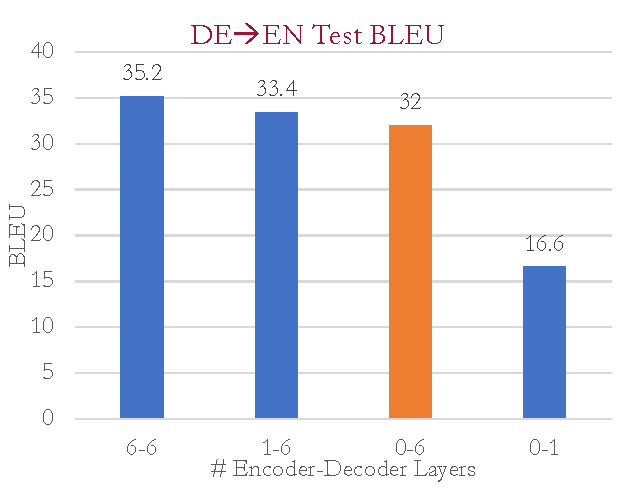
\includegraphics[width=0.45\linewidth]{img/misc/noencoder.deen.pdf}
     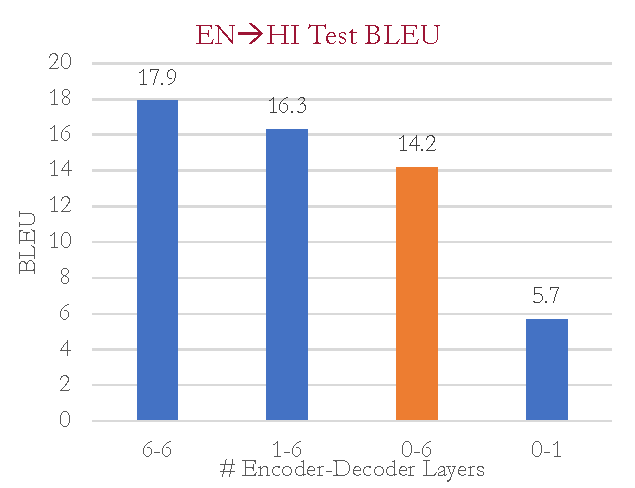
\includegraphics[width=0.45\linewidth]{img/misc/noencoder.enhi.pdf}
     
     \caption{Caption}
     \label{fig:my_label}
 \end{figure}
 
 
 
 